\documentclass[a4paper,12pt]{article}

\usepackage[utf8]{inputenc}
\usepackage{geometry}

\geometry{
    left=1cm,
    right=1cm,
    top=1.5cm,
    bottom=2.5cm
}

\usepackage{setspace}
\usepackage{tikz}
\usepackage{tkz-graph}
\usetikzlibrary{trees}

\definecolor{lightblue}{RGB}{182, 249, 255}
\definecolor{darkblue}{RGB}{19, 75, 95}
\definecolor{bluedot}{RGB}{81,171,203}

\begin{document}

\begin{center}
    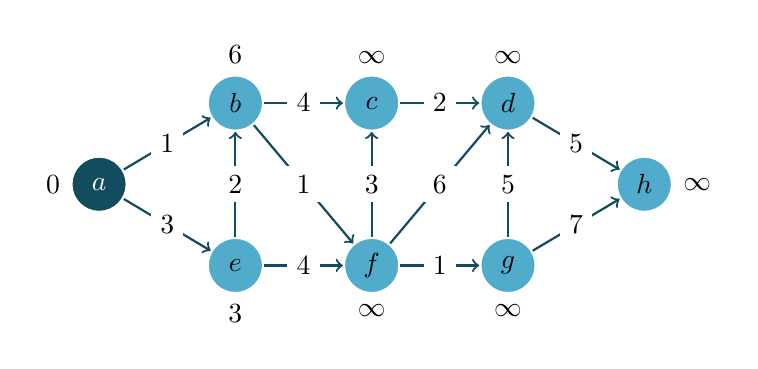
\begin{tikzpicture}[thick, main/.style = {draw=white, text=black, circle, fill=bluedot,rounded corners=0.5mm,minimum size=2em}, scale=0.2,
        selected/.style = {draw=white, text=white, circle, fill=darkblue,rounded corners=0.5mm,minimum size=2em},
        EdgeStyle/.append style = {->, draw=darkblue, thick}]
        \matrix [column sep=1cm, row sep=0.3cm]{
                           & \node[main,label=above:{$6$}] (2) {$b$}; & \node[main,label=above:{$\infty$}] (5) {$c$}; & \node[main,label=above:{$\infty$}] (8) {$d$};  &  \\
    \node[selected,label=left:{$0$}] (1) {$a$}; & & & & \node[main,label=right:{$\infty$}] (11) {$h$}; \\ 
     & \node[main,label=below:{$3$}] (3) {$e$}; & \node[main,label=below:{$\infty$}] (6) {$f$}; & \node[main,label=below:{$\infty$}] (9) {$g$}; \\ 
    };
    \draw[] (1) (2);
    \Edge[label = 1](1)(2)
    \draw[] (1) (3);
    \Edge[label = 3](1)(3)
    \draw[] (2) (3);
    \Edge[label = 2](3)(2)
    \draw[] (2) (5);
    \Edge[label = 4](2)(5)
    \draw[] (3) (6);
    \Edge[label = 4](3)(6)
    \draw[] (5) (6);
    \Edge[label = 3](6)(5)
    \draw[] (5) (8);
    \Edge[label = 2](5)(8)
    \draw[] (6) (9);
    \Edge[label = 1](6)(9)
    \draw[] (2) (6);
    \Edge[label = 1](2)(6)
    \draw[] (6) (8);
    \Edge[label = 6](6)(8)
    \draw[] (8) (9);
    \Edge[label = 5](9)(8)
    \draw[] (8) (11);
    \Edge[label = 5](8)(11)
    \draw[] (9) (11);
    \Edge[label = 7](9)(11)
    \end{tikzpicture}
\end{center}
    
\end{document}